% Western Themed Beamer

\documentclass[12pt,ignorenonframetext,]{beamer}
\setbeamertemplate{caption}[numbered]
\setbeamertemplate{caption label separator}{:}
\setbeamercolor{caption name}{fg=normal text.fg}
\usepackage{amssymb,amsmath}
\usepackage{ifxetex,ifluatex}
\usepackage{fixltx2e} % provides \textsubscript
\usepackage{lmodern}
\ifxetex
\usepackage{fontspec,xltxtra,xunicode}
\defaultfontfeatures{Mapping=tex-text,Scale=MatchLowercase}
\newcommand{\euro}{€}
\else
\ifluatex
\usepackage{fontspec}
\defaultfontfeatures{Mapping=tex-text,Scale=MatchLowercase}
\newcommand{\euro}{€}
\else
\usepackage[T1]{fontenc}
\usepackage[utf8]{inputenc}
\fi
\fi
% use upquote if available, for straight quotes in verbatim environments
\IfFileExists{upquote.sty}{\usepackage{upquote}}{}
% use microtype if available
\IfFileExists{microtype.sty}{\usepackage{microtype}}{}

\setlength{\parindent}{0pt}
\setlength{\parskip}{6pt plus 2pt minus 1pt}
\setlength{\emergencystretch}{3em}  % prevent overfull lines
\providecommand{\tightlist}{%
	\setlength{\itemsep}{0pt}\setlength{\parskip}{0pt}}
\setcounter{secnumdepth}{0}

%%Color Themes
\usepackage{xcolor}
\definecolor{helmuth}{RGB}{79, 38, 131/250} % 
\definecolor{westernSilver}{RGB}{128,127,131} %

\usetheme{Madrid}
\useoutertheme{miniframes}\useinnertheme{circles}
\setbeamertemplate{navigation symbols}{}
%Set Beamer Colors
\setbeamercolor{palette primary}{bg=helmuth,fg=white}
\setbeamercolor{palette secondary}{bg=helmuth,fg=white}
\setbeamercolor{palette tertiary}{bg=helmuth,fg=white}
\setbeamercolor{palette quaternary}{bg=helmuth,fg=white}
\setbeamercolor{structure}{fg=helmuth} % itemize, enumerate, etc
\setbeamercolor{section in toc}{fg=helmuth} % TOC sections
\setbeamercolor*{titlelike}{fg=white,bg=helmuth}
\setbeamercolor{subsection in head/foot}{bg=westernSilver,fg=white}
\setbeamercolor{itemize item}{fg=black}
\setbeamercolor{enumerate item}{fg=black}

\setbeamertemplate{itemize items}[default]
\setbeamertemplate{enumerate items}[default]



%% Beamer Behaviour
\AtBeginPart{}
\AtBeginSection{}
\AtBeginSubsection{}
\AtBeginSubsubsection{}
\setlength{\emergencystretch}{0em}
\setlength{\parskip}{0pt}



%% Front matter conditionals.
\title[Stats for ML]{Basic Statistics for Machine Learning}
\subtitle{You Could Call It ``Statistical Learning''}
\author[
D.Pananos
]{Demetri Pananos}
\institute[
]{
		
\includegraphics[width=15mm,keepaspectratio]{../western.png}\\
	\vspace{2 mm}
			Department of Epidemiology \& Biostatistics \newline Schulich School of
Medicine \& Dentistry \\
		Western University
	}


\logo{
						
\includegraphics[width=7.5mm,keepaspectratio]{../western.png}
		}


\date[
2018-10-31
]{
		2018-10-31
			}


\begin{document}

\begin{frame}[plain]
\titlepage
\end{frame}

\hypertarget{introduction}{%
\subsection{Introduction}\label{introduction}}

\begin{frame}{I Have A Problem}
\protect\hypertarget{i-have-a-problem}{}

\begin{center}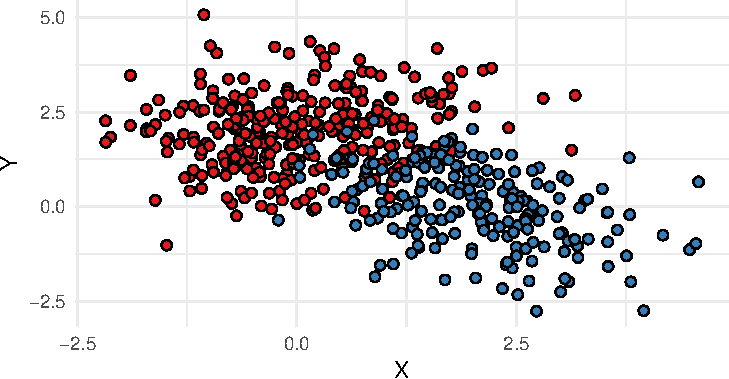
\includegraphics{CSS_Presentation_files/figure-beamer/unnamed-chunk-1-1} \end{center}

\end{frame}

\begin{frame}{I Have a Problem}
\protect\hypertarget{i-have-a-problem-1}{}

\begin{center}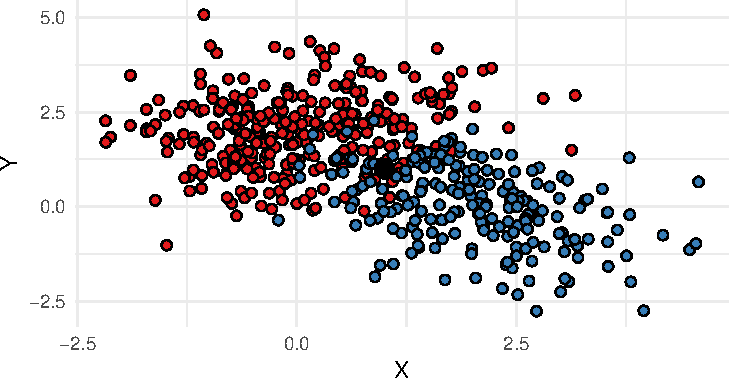
\includegraphics{CSS_Presentation_files/figure-beamer/unnamed-chunk-2-1} \end{center}

\end{frame}

\begin{frame}{How Can I Solve It?}
\protect\hypertarget{how-can-i-solve-it}{}

\begin{itemize}
\item
  We can do this in a variety of ways.
\item
  Some are very statistical. Some are very complicated.
\item
  Some are in the middle. I'll call those \emph{statistical learning
  algorithms}.
\end{itemize}

\end{frame}

\begin{frame}{Statistical Decision Theory}
\protect\hypertarget{statistical-decision-theory}{}

\begin{itemize}
\item
  The ``Theorectically Optimal'' way to do this would require knowing
  \(P( \mbox{Is Red} \vert X,Y)\).
\item
  Maybe approximating this conditional distribution will be enough.
\item
  But first, a little vocabularty
\end{itemize}

\end{frame}

\hypertarget{probability}{%
\subsection{Probability}\label{probability}}

\begin{frame}{Vocabulary}
\protect\hypertarget{vocabulary}{}

\begin{center}
Marginal $$P(X)$$

Joint $$P(X,Y)$$

Conditional $$P(X \vert Y)$$
\end{center}

\end{frame}

\begin{frame}{Probability}
\protect\hypertarget{probability-1}{}

Sum Rule

\[P(X) = \sum_Y P(X,Y)\]

Product/Chain Rule

\[P(X,Y) = P(Y|X)P(X) \overset{or}{=} P(X|Y)P(Y)\]

\end{frame}

\begin{frame}{Probability}
\protect\hypertarget{probability-2}{}

We can recover some very powerful rules just from these. For example,
Bayes' Rule

\[P(Y|X) = \dfrac{P(X|Y)P(Y)}{\displaystyle{\sum_Y} P(X|Y)P(Y) }\]

\end{frame}

\begin{frame}{Naive Bayes}
\protect\hypertarget{naive-bayes}{}

Use Bayes' Theorem to compute \(P(\mbox{Is Red}|X,Y)\).

\[P(\mbox{Is Red}|X,Y) \propto P(\mbox{Is Red})P(X,Y|\mbox{Is Red})\]

\end{frame}

\begin{frame}{Naive Bayes}
\protect\hypertarget{naive-bayes-1}{}

\[P(\mbox{Is Red}) = \mbox{The proportion of our sample which belongs to } \mbox{ Red} \]

\[P(X,Y|\mbox{Is Red}) = \mbox{Distribution of data belonging to } \mbox{Red}\]

\end{frame}

\begin{frame}{The Naive Part}
\protect\hypertarget{the-naive-part}{}

The Naive Part of Naive Bayes

\[P(X,Y|\mbox{Is Red}) = P(X \vert \mbox{Is Red})P(Y\vert \mbox{Is Red})\]

\end{frame}

\begin{frame}{All in All}
\protect\hypertarget{all-in-all}{}

\[P(\mbox{Is Red}|X,Y) = P(\mbox{Is Red})P(X \vert \mbox{Is Red})P(Y\vert\mbox{Is Red})\]

Make another assumption that \(P(X \vert \mbox{Is Red})\) is normal.

\end{frame}

\begin{frame}{}
\protect\hypertarget{section}{}

\begin{center}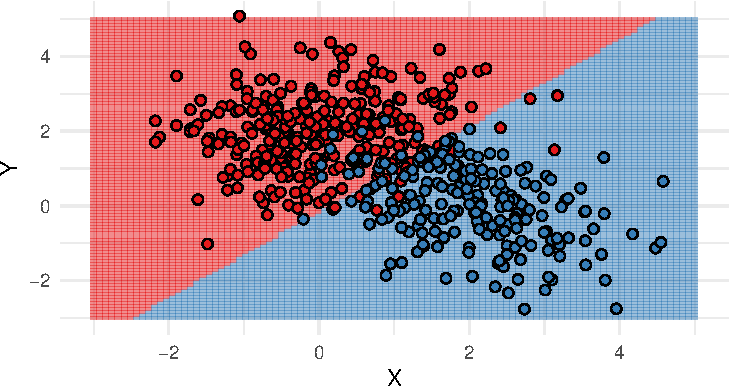
\includegraphics{CSS_Presentation_files/figure-beamer/unnamed-chunk-3-1} \end{center}

\end{frame}

\begin{frame}{}
\protect\hypertarget{section-1}{}

\begin{center}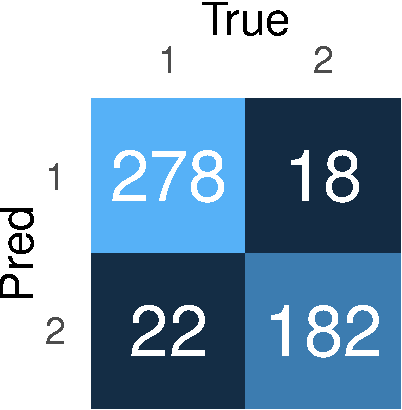
\includegraphics{CSS_Presentation_files/figure-beamer/unnamed-chunk-4-1} \end{center}

\end{frame}

\hypertarget{quadratic-discriminant-analysis}{%
\subsection{Quadratic Discriminant
Analysis}\label{quadratic-discriminant-analysis}}

\begin{frame}{Quadratic Discriminant Analysis}
\protect\hypertarget{quadratic-discriminant-analysis-1}{}

Naive Bayes ignores the covariance between data by assuming independence
between covariates.

Quadratic Discriminant Analysis will use some information about
covariance to help make predictions. In order to fit these models, we
need to understand

\begin{itemize}
\tightlist
\item
  Expectation in \(\mathbb{R}^n\)
\item
  Covariance Matrices
\end{itemize}

\end{frame}

\begin{frame}{Means and Covariance}
\protect\hypertarget{means-and-covariance}{}

\begin{itemize}
\item
  Expectations in multiple dimenions behave like expectations in a
  single variable.
\item
  If \(X\) is an \(n\)-dimensional random variable with expectation
  \(\boldsymbol{\mu}\), then
\end{itemize}

\[ E[X] =  \boldsymbol{\mu} = \begin{bmatrix} \mu_1 \\ \mu_2 \\ \vdots \\ \mu_n  \end{bmatrix} \approx \begin{bmatrix} \sum_k \dfrac{x_{1k}}{N}  \\ \vdots \\ \sum_k \dfrac{x_{nk}}{N} \end{bmatrix} \]

\end{frame}

\begin{frame}{Means and Covariance}
\protect\hypertarget{means-and-covariance-1}{}

\begin{itemize}
\tightlist
\item
  If \(X\) is an \(n\)-dimensional random variable with covariance
  matrix \(\Sigma\), then
\end{itemize}

\[\Sigma_{ij} = \operatorname{Cov}(X_i,X_j) \].

\begin{itemize}
\tightlist
\item
  This implies \(\Sigma^T = \Sigma\) since the covariance is a symmetric
  operator.
\end{itemize}

\end{frame}

\begin{frame}{Back To Quadratic Discriminant Analysis}
\protect\hypertarget{back-to-quadratic-discriminant-analysis}{}

\begin{itemize}
\item
  Assume that
  \(X | C_k \sim \mathcal{N}(\boldsymbol{\mu}_k, \Sigma_k)\). That is,
  assume that the two classes have different covariance and different
  means.
\item
  Compute \(P(C = C_k | X)\) using Baye's rule.
\end{itemize}

\end{frame}

\begin{frame}{}
\protect\hypertarget{section-2}{}

\begin{center}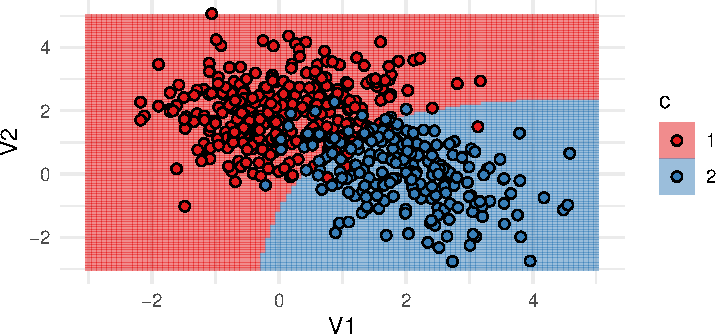
\includegraphics{CSS_Presentation_files/figure-beamer/unnamed-chunk-5-1} \end{center}

\end{frame}

\begin{frame}{}
\protect\hypertarget{section-3}{}

\begin{center}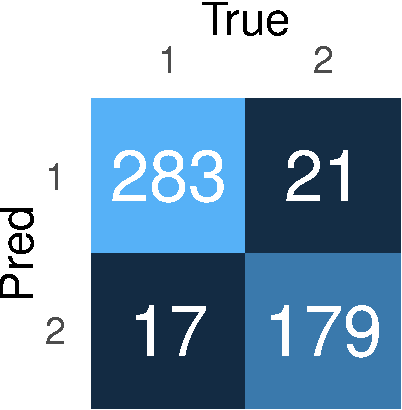
\includegraphics{CSS_Presentation_files/figure-beamer/unnamed-chunk-6-1} \end{center}

\end{frame}

\begin{frame}{What Have We Seen?}
\protect\hypertarget{what-have-we-seen}{}

\begin{itemize}
\tightlist
\item
  A little statistics can get you very far.
\end{itemize}

\end{frame}



\end{document}